\documentclass[10pt,journal,compsoc]{IEEEtran}
\usepackage[utf8]{inputenc}
\usepackage{amsmath} % align environment
\usepackage{amssymb} % mathbb
\usepackage{bussproofs} % notation for inference rules
\usepackage{rotating} % sidewaysfigure
\usepackage[hyphens]{url}
\usepackage{hyperref}
\usepackage[nocompress]{cite}

% Theorem environments
\usepackage{amsthm}
\newtheorem{definition}{Definition}
\newtheorem{theorem}{Theorem}
\newtheorem{lemma}[theorem]{Lemma}
\newtheorem*{convergence-thm}{Theorem}

% Diagrams
\usepackage{tikz}
\usetikzlibrary{arrows}

\hyphenation{da-ta-cen-ter da-ta-cen-ters net-works time-stamp}

\newif\ifproofdraft
\proofdraftfalse

\newcommand{\evalto}{\;\Longrightarrow\;}

% Placeholder character like \textvisiblespace, but works in math mode
\newcommand{\placeholder}{%
  \makebox[0.7em]{%
    \kern.07em
    \vrule height.3ex
    \hrulefill
    \vrule height.3ex
    \kern.07em
  }%
}

% Span multiple columns within an alignat math environment
\newcommand{\multialign}[2]{%
  \multispan{#1}\mbox{$\displaystyle{}#2$}%
}

\begin{document}
\sloppy
\title{A Conflict-Free Replicated JSON Datatype}
\author{Author 1 and Author 2
\thanks{Author affiliation goes here.}}

\IEEEtitleabstractindextext{%
\begin{abstract}
% abstract word limit: 100-200 words
Many applications model their data in a general-purpose storage format such as JSON. This data structure is modified by the application as a result of user input. Such modifications are well understood if performed sequentially on a single copy of the data, but the semantics is unclear if the data is replicated and modified concurrently on multiple devices. In this paper we present an algorithm and formal semantics for a JSON data structure that automatically resolves concurrent modifications such that no updates are lost, and such that all replicas converge towards the same state. It supports arbitrarily nested list and map types, which can be modified by insertion, deletion and assignment. The algorithm performs all merging client-side and does not depend on ordering guarantees from the network, allowing it to be deployed in peer-to-peer networks and in messaging systems with end-to-end encryption.
\end{abstract}

\begin{IEEEkeywords}
CRDTs, Collaborative Editing, P2P, JSON, Optimistic Replication, Semantics, Eventual Consistency.
\end{IEEEkeywords}}
\maketitle

\IEEEraisesectionheading{\section{Introduction}\label{sec:introduction}}

\IEEEPARstart{U}{sers} of mobile devices, such as smartphones, expect applications to continue working while the device is offline or has poor network connectivity, and to synchronize its state with the user's other devices when the network is available. Examples of such applications include calendars, address books, note-taking tools, to-do lists, and password managers. Moreover, many people want to collaborate with others on text documents, spreadsheets, presentations, graphics, and other kinds of document.

What these applications have in common is that the application state needs to be replicated to several devices, each of which may modify the state locally. Requiring serializability, the traditional approach to concurrency control, would cause the application to become unusable at times of poor network connectivity~\cite{Davidson:1985hv}. If we require that applications work regardless of the network, we must assume that users can make arbitrary modifications concurrently on different devices, and that any resulting conflicts must be resolved.

The simplest way of resolving conflicts is to discard some document modifications if a conflict occurred, for example using a ``last writer wins'' policy. However, this approach is undesirable as it incurs data loss. An alternative is to let the user manually resolve the conflict, which is tedious in case of modifications that could be merged automatically.

Current applications solve this problem with a range of ad-hoc and application-specific mechanisms. In this paper we present a general-purpose datatype that provides the full expressiveness of the JSON data model, and automatically merges any concurrent modifications without loss of information. We expect that implementations of this datatype will drastically simplify the development of collaborative and state-synchronizing applications for mobile devices.

\subsection{JSON data model}

JSON is a popular general-purpose data encoding format, used in many databases and web services. It has similarities to XML, and we compare them in Section~\ref{sec:json-xml}. The structure of a JSON document can optionally be constrained by a schema; however, for simplicity, this paper discusses only untyped JSON without an explicit schema.

A JSON document is a tree containing two types of branch node:

\begin{description}
\item[Map:] A node whose children have no defined order, and where each child is labelled with a string \emph{key}. A key uniquely identifies one of the children. We treat keys as immutable, but values as mutable, and key-value mappings can be added and removed from the map. A JSON map is also known as an \emph{object}.
\item[List:] A node whose children have an order defined by the application. The list can be mutated by inserting or deleting list elements. A JSON list is also known as an \emph{array}.
\end{description}

A child of a branch node can be either another branch node, or a leaf node. A leaf of the tree contains a primitive value (string, number, boolean, or null). We treat primitive values as immutable, but allow the value of a leaf node to be modified by treating it as a \emph{register} that can be assigned a new value.

This model is sufficient to express the state of a wide range of applications. For example, a text document can be represented by a list of single-character strings; character-by-character edits are then expressed as insertions and deletions of list elements. In Section~\ref{sec:examples} we show further examples of using JSON to model application data.

\subsection{Replication and conflict resolution}\label{sec:intro-replication}

We consider systems in which a full copy of the JSON document is replicated on several devices. Those devices could be servers in datacenters, but we focus on mobile devices such as smartphones and laptops, which have intermittent network connectivity. We do not distinguish between devices owned by the same user and different users. Our model allows each device to optimistically modify its local replica of the document, and to asynchronously propagate those edits to other replicas.

Our only requirement of the network is that messages sent by one replica are eventually delivered to all other replicas, by retrying if delivery fails. We assume the network may arbitrarily delay, reorder and duplicate messages.

Our algorithm works client-side and does not depend on any server to transform or process messages. This approach allows messages to be delivered via a peer-to-peer network and a secure messaging protocol with end-to-end encryption~\cite{Unger:2015kg}, although the details of the network implementation and cryptographic protocols are outside of the scope of this paper.

In Section~\ref{sec:semantics} we give a formal semantics that describes how conflicts are resolved when a JSON document is concurrently modified on different devices. Our design is based on three simple principles:
\begin{enumerate}
\item All replicas of the data structure should automatically converge towards the same state.
\item No user input should be lost due to concurrent modifications.
\item If all sequential permutations of a set of updates lead to the same state, then concurrent execution of those updates also leads to the same state~\cite{Bieniusa:2012gt}.
\end{enumerate}

\subsection{Our contributions}

Our main contribution in this work is to define an algorithm and formal semantics for collaborative, concurrent editing of JSON data structures with automatic conflict resolution. Although similar algorithms have previously been defined for lists, maps and registers individually (see Section~\ref{sec:related}), to our knowledge this paper is the first to integrate all of these structures into an arbitrarily composable datatype.

Composing maps and lists into arbitrarily nested structures opens up subtle challenges that do not arise in flat structures, due to the possibility of concurrent edits at different levels of the tree. We illustrate some of those challenges by example in Section~\ref{sec:examples}. On the other hand, nested structures are an important requirement for many applications; by providing an algorithm that handles conflict resolution on such structures, we hope to simplify the the development of applications that use optimistic replication.

\section{Related work}\label{sec:related}

In this section we discuss existing approaches to optimistic replication, collaborative editing and conflict resolution.

\subsection{Operational transformation}\label{sec:related-ot}

Algorithms based on \emph{operational transformation} (OT) have long been used for collaborative editing applications~\cite{Ellis:1989ue,Ressel:1996wx,Sun:1998vf,Nichols:1995fd}. Most of them treat a document as a single ordered list (of characters, for example) and do not support the nested tree structures that are required for many applications. Some algorithms generalize OT to editing XML documents~\cite{Davis:2002iv,Ignat:2003jy,Wang:2015vo}, which provides nesting of ordered lists, but these algorithms do not support key-value maps as defined in this paper (see Section~\ref{sec:json-xml}). The performance of OT algorithms degrades rapidly as the number of concurrent operations increases~\cite{Li:2006kd}.

Most deployed OT collaboration systems, including Google Docs~\cite{DayRichter:2010tt}, Etherpad~\cite{Etherpad:2011um}, Novell Vibe~\cite{Spiewak:2010vw} and Apache Wave (formerly Google Wave~\cite{Wang:2015vo}), rely on a single server to decide on a total ordering of operations~\cite{Lemonik:2016wh}, a design decision inherited from the Jupiter system~\cite{Nichols:1995fd}. This approach has the advantage of making the transformation functions simpler and less error-prone~\cite{Imine:2003ks}, but it does not meet our requirements, since we want to support peer-to-peer collaboration without requiring a single server.

Many secure messaging protocols, which we plan to use for encrypted collaboration, do not guarantee that different recipients will see messages in the same order~\cite{Unger:2015kg}. Although it is possible to decide on a total ordering of operations by using an atomic broadcast protocol~\cite{Defago:2004ji}, which avoids relying on a single server, such protocols are equivalent to consensus~\cite{Chandra:1996cp}, so they can only safely make progress if a majority of participants are online and reachable. We expect that in peer-to-peer systems of mobile devices it will frequently be the case that only a minority of participants are online at the same time, and so any algorithm requiring atomic broadcast would become unavailable. The strongest guarantee such a system can give is causal ordering~\cite{Attiya:2015dm}.

The Google Realtime API~\cite{Google:2015vk} is to our knowledge the only implementation of OT that supports arbitrary nesting of lists and maps. Like Google Docs, it relies on a single server~\cite{Lemonik:2016wh}. As a proprietary product, details of its algorithms have not been published.

\subsection{CRDTs}\label{sec:related-crdts}

Conflict-free replicated datatypes (CRDTs) are a family of data structures that can be concurrently modified and that guarantee convergence of such concurrent updates. They work by attaching additional metadata to the data structure, and making modification operations commutative by construction. The JSON datatype described in this paper is a kind of CRDT.

CRDTs for registers, counters, maps and sets are widely known~\cite{Shapiro:2011un,Shapiro:2011wy}, and have been implemented in various deployed systems such as Riak~\cite{Brown:2014hs,Brown:2013wy}. For ordered lists, various algorithms have been proposed, including WOOT~\cite{Oster:2006wj}, RGA~\cite{Roh:2011dw}, Treedoc~\cite{Preguica:2009fz}, Logoot~\cite{Weiss:2010hx} and LSEQ~\cite{Nedelec:2013ky}. However, none of them support nesting: they assume that the elements of the CRDT map or list are primitive values, not another CRDT.

The problem of nesting one CRDT inside another (also known as \emph{composition} or \emph{embedding}) has only been studied more recently. Riak allows nesting of counters and registers inside maps, and of maps within other maps~\cite{Brown:2014hs,Brown:2013wy}. Embedding counters inside maps raises questions of semantics, which have been studied by Baquero, Almeida and Lerche~\cite{Baquero:2016iv}. Almeida et al.~\cite{Almeida:2016tk} also define delta mutations for nested maps, and Baquero et al.~\cite{Baquero:2015tm} define a theoretical framework for composition of state-based CRDTs, based on lattices. None of this work integrates CRDTs for ordered lists, but the treatment of causality in these datatypes forms a basis for the semantics developed in this paper.

Burckhardt et al.~\cite{Burckhardt:2012jy} define \emph{cloud types}, which are similar to CRDTs and can be composed. They define \emph{cloud arrays}, which behave similarly to our map datatype, and \emph{entities}, which are like unordered sets or relations; ordered lists are not defined in this framework.

Although CRDTs for registers, maps and ordered lists have existed for years in isolation, we are not aware of any prior work that allows them all to be composed into an arbitrarily nested CRDT with a JSON-like structure.

\subsection{Other approaches}\label{sec:related-other}

Many replicated data systems need to deal with the problem of concurrent, conflicting modifications, but the solutions are often ad-hoc. For example, in Dynamo~\cite{DeCandia:2007ui}, if several values are concurrently written to the same key, the database preserves all of these values, and leaves conflict resolution to application code. Naively chosen merge functions often exhibit anomalies such as deleted items reappearing~\cite{DeCandia:2007ui}. We believe that conflict resolution is not a simple matter that can reasonably be left to application programmers.

Another frequently-used approach to conflict resolution is \emph{last writer wins} (LWW), which arbitrarily chooses one among several concurrent writes as ``winner'' and discards the others. This approach is used in Apache Cassandra, and it is an option in many other systems including Riak and CouchDB. LWW does not meet our requirements, since we want no user input to be lost due to concurrent modifications.

Finally, systems such as Bayou~\cite{Terry:1995dn} allow offline nodes to execute transactions tentatively, and confirm them when they are next online. This approach relies on all servers executing transactions in the same serial order, and deciding whether a transaction was successful depending on its preconditions. As discussed in Section~\ref{sec:related-ot}, such serial ordering requirements are prohibitive in a peer-to-peer system of mobile devices. The possibility of tentative transactions later being rolled back also opens the risk of user input being lost.


\section{Composing data structures}\label{sec:composing}

In this section we informally introduce our approach to collaborative editing of JSON data structures. A formal presentation of the algorithm follows in Section~\ref{sec:semantics}.

\subsection{Concurrent editing examples}\label{sec:examples}

\begin{figure}
\centering
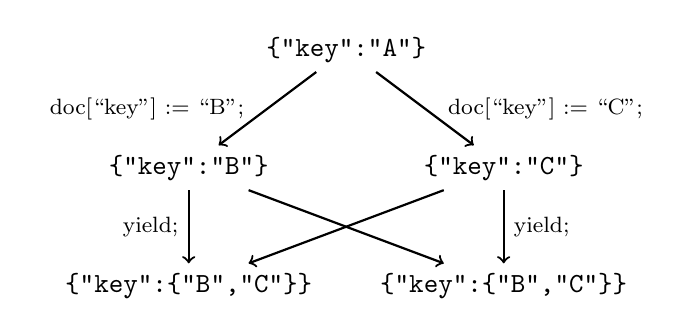
\begin{tikzpicture}[auto]
\node (start)  at (2,3) {\verb|{"key":"A"}|};
\node (left1)  at (0,1.5) {\verb|{"key":"B"}|};
\node (right1) at (4,1.5) {\verb|{"key":"C"}|};
\node (left2)  at (0,0) {\verb|{"key":{"B","C"}}|};
\node (right2) at (4,0) {\verb|{"key":{"B","C"}}|};
\draw [thick,->] (start) to node [left,inner sep=8pt] {\footnotesize doc[``key''] := ``B'';} (left1);
\draw [thick,->] (start) to node [right,inner sep=8pt] {\footnotesize doc[``key''] := ``C'';} (right1);
\draw [thick,->] (left1) to node [left] {\footnotesize yield;} (left2);
\draw [thick,->] (left1) to (right2);
\draw [thick,->] (right1) to (left2);
\draw [thick,->] (right1) to node [right] {\footnotesize yield;} (right2);
\end{tikzpicture}
\caption{Concurrent assignment to a register.}\label{fig:register-assign}
\end{figure}

To illustrate some of the subtleties that arise when JSON documents are concurrently modified, we present some examples.

Our first example is shown in Figure~\ref{fig:register-assign}. In a document that maps ``key'' to a register with value ``A'', one replica sets the value of the register to ``B'', while another concurrently sets it to ``C''. As the replicas subsequently exchange edits, they detect the conflict. Since we do not want to simply discard one of the edits, and the strings ``B'' and ``C'' cannot meaningfully be merged, the system must preserve both concurrent updates. This datatype is known as a \emph{multi-value register}: although a replica can only assign a single value to the register, reading the register may return a set of multiple values that were concurrently written. An implementation may keep metadata about the provenance of each value (who made the change, on which device, at what time) to assist users with manually resolving the conflict.

\begin{figure*}
\centering
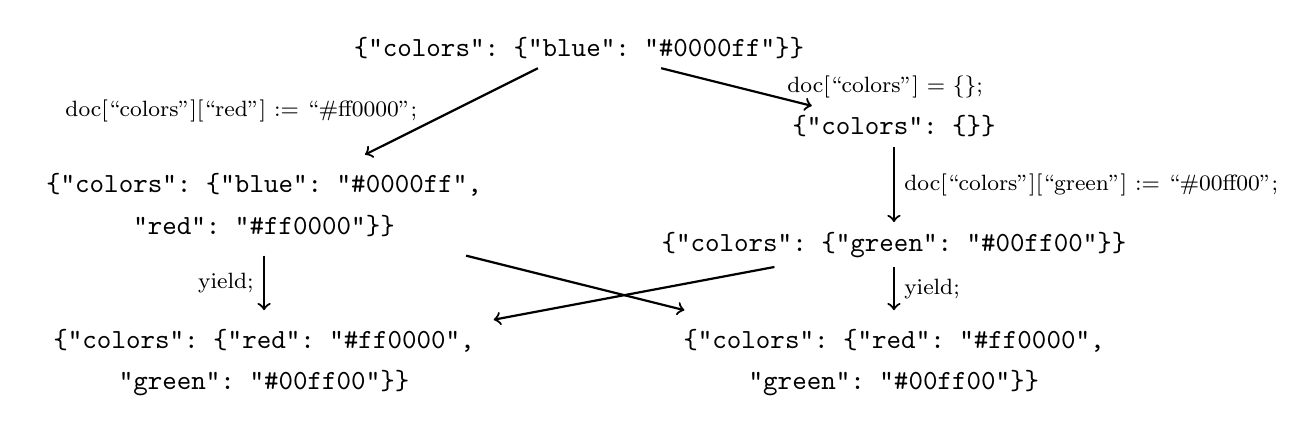
\begin{tikzpicture}[auto]
\node (start) at (4,4) {\verb|{"colors": {"blue": "#0000ff"}}|};
\node [matrix] (left1) at (0,2) {
    \node {\verb|{"colors": {"blue": "#0000ff",|}; \\
    \node {\verb|"red": "#ff0000"}}|}; \\
};
\node (right1) at (8,3) {\verb|{"colors": {}}|};
\node (right2) at (8,1.5) {\verb|{"colors": {"green": "#00ff00"}}|};
\node [matrix] (left2) at (0,0) {
    \node {\verb|{"colors": {"red": "#ff0000",|}; \\
    \node {\verb|"green": "#00ff00"}}|}; \\
};
\node [matrix] (right3) at (8,0) {
    \node {\verb|{"colors": {"red": "#ff0000",|}; \\
    \node {\verb|"green": "#00ff00"}}|}; \\
};
\draw [thick,->] (start)  to node [left, inner xsep=12pt] {\footnotesize doc[``colors''][``red''] := ``\#ff0000'';} (left1);
\draw [thick,->] (start)  to node [right,inner xsep=18pt] {\footnotesize doc[``colors''] = \{\};} (right1);
\draw [thick,->] (right1) to node [right] {\footnotesize doc[``colors''][``green''] := ``\#00ff00'';} (right2);
\draw [thick,->] (left1)  to node [left]  {\footnotesize yield;} (left2);
\draw [thick,->] (right2) to node [right] {\footnotesize yield;} (right3);
\draw [thick,->] (left1)  to (right3);
\draw [thick,->] (right2) to (left2);
\end{tikzpicture}
\caption{Modifying the contents of a nested map while concurrently the entire map is overwritten.}\label{fig:map-remove}
\end{figure*}

Another example is given in Figure~\ref{fig:map-remove}. Here, one replica adds ``red'' to a map of colors, while concurrently another client first blanks out the entire map of colors, and then adds ``green''. As the replicas merge their edits, all changes must be preserved: ``blue'' must be absent from the final map, since it was removed by blanking out the map, while ``red'' and ``green'' must be present, since they were explicitly added.

\begin{figure*}
\centering
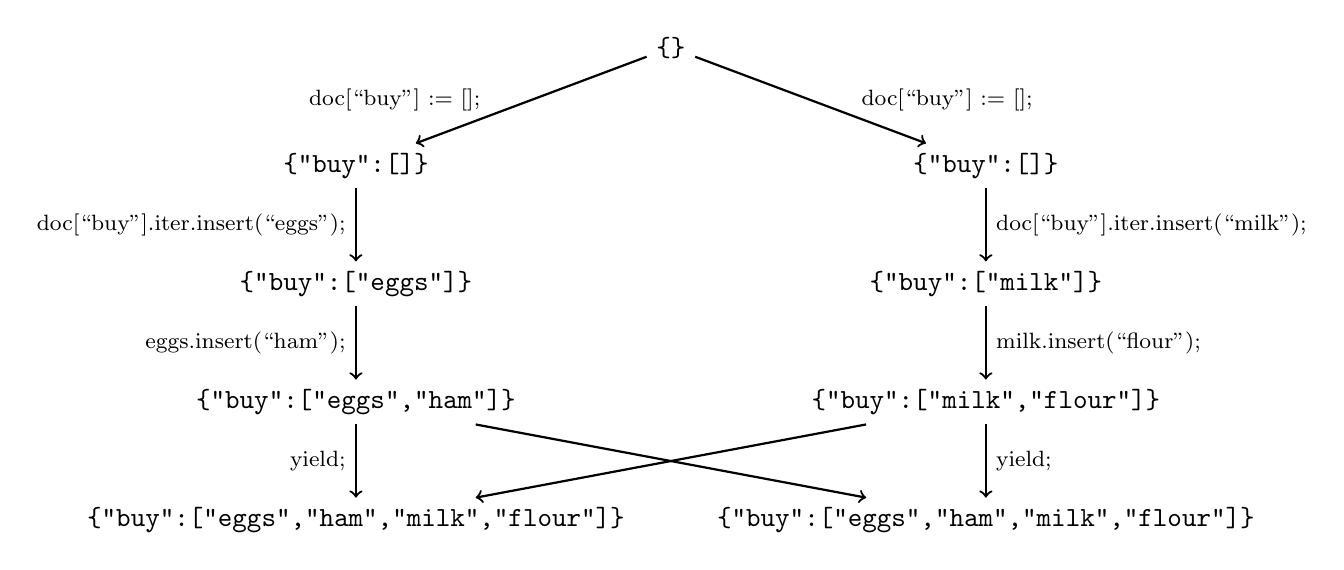
\begin{tikzpicture}[auto]
\node (start)  at (4,6.0) {\verb|{}|};
\node (left1)  at (0,4.5) {\verb|{"buy":[]}|};
\node (right1) at (8,4.5) {\verb|{"buy":[]}|};
\node (left2)  at (0,3.0) {\verb|{"buy":["eggs"]}|};
\node (left3)  at (0,1.5) {\verb|{"buy":["eggs","ham"]}|};
\node (right2) at (8,3.0) {\verb|{"buy":["milk"]}|};
\node (right3) at (8,1.5) {\verb|{"buy":["milk","flour"]}|};
\node (left4)  at (0,0.0) {\verb|{"buy":["eggs","ham","milk","flour"]}|};
\node (right4) at (8,0.0) {\verb|{"buy":["eggs","ham","milk","flour"]}|};
\draw [thick,->] (start)  to node [left, inner xsep=18pt] {\footnotesize doc[``buy''] := [];} (left1);
\draw [thick,->] (start)  to node [right,inner xsep=18pt] {\footnotesize doc[``buy''] := [];} (right1);
\draw [thick,->] (left1)  to node [left]  {\footnotesize doc[``buy''].iter.insert(``eggs'');} (left2);
\draw [thick,->] (right1) to node [right] {\footnotesize doc[``buy''].iter.insert(``milk'');} (right2);
\draw [thick,->] (left2)  to node [left]  {\footnotesize eggs.insert(``ham'');} (left3);
\draw [thick,->] (right2) to node [right] {\footnotesize milk.insert(``flour'');} (right3);
\draw [thick,->] (left3)  to node [left]  {\footnotesize yield;} (left4);
\draw [thick,->] (right3) to node [right] {\footnotesize yield;} (right4);
\draw [thick,->] (left3)  to (right4);
\draw [thick,->] (right3) to (left4);
\end{tikzpicture}
\caption{Two replicas concurrently create ordered lists under the same map key.}\label{fig:two-lists}
\end{figure*}

The example in Figure~\ref{fig:two-lists} shows two replicas concurrently creating a new shopping list under the same map key ``buy'', and adding items to the list. When the replicas are merged, the lists need to be merged also. We preserve the ordering and adjacency of items inserted at each replica, so ``ham'' appears after ``eggs'', and ``flour'' appears after ``milk'' in the merged result. There is no information on which replica's items should appear first in the merged result, so the algorithm can make an arbitrary choice between ``eggs, ham, milk, flour'' and ``milk, flour, eggs, ham'', provided that all replicas end up with the same order.

\begin{figure*}
\centering
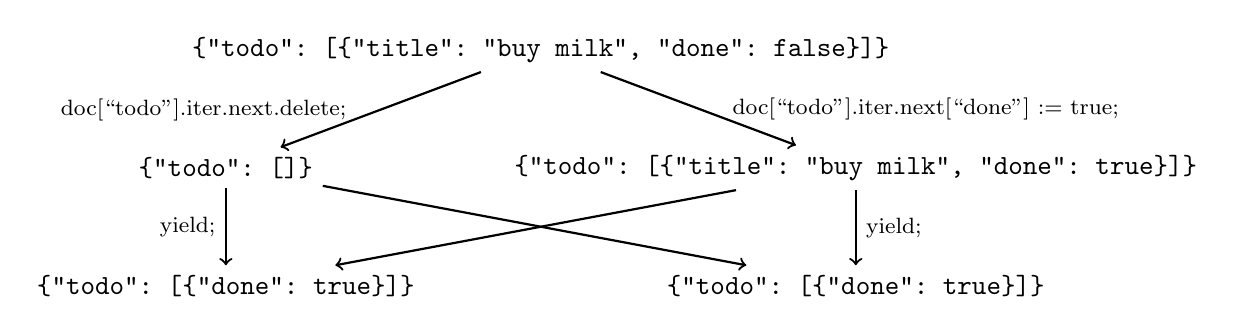
\begin{tikzpicture}[auto]
\node (start)  at (4,3.0) {\verb|{"todo": [{"title": "buy milk", "done": false}]}|};
\node (left1)  at (0,1.5) {\verb|{"todo": []}|};
\node (right1) at (8,1.5) {\verb|{"todo": [{"title": "buy milk", "done": true}]}|};
\node (left2)  at (0,0.0) {\verb|{"todo": [{"done": true}]}|};
\node (right2) at (8,0.0) {\verb|{"todo": [{"done": true}]}|};
\draw [thick,->] (start)  to node [left, inner xsep=12pt] {\footnotesize doc[``todo''].iter.next.delete;} (left1);
\draw [thick,->] (start)  to node [right,inner xsep=12pt] {\footnotesize doc[``todo''].iter.next[``done''] := true;} (right1);
\draw [thick,->] (left1)  to node [left]  {\footnotesize yield;} (left2);
\draw [thick,->] (right1) to node [right] {\footnotesize yield;} (right2);
\draw [thick,->] (left1)  to (right2);
\draw [thick,->] (right1) to (left2);
\end{tikzpicture}
\caption{One replica removes a list element, while another concurrently updates its contents.}\label{fig:todo-item}
\end{figure*}

Our final example in Figure~\ref{fig:todo-item} shows a limitation of the principle of preserving all user input. In a to-do list application, one replica removes a to-do item from the list, while another replica concurrently marks the same item as done. As the changes are merged, the update of the map key ``done'' effectively causes the list item to be resurrected on the left replica, leading to a to-do item without a title (since the title was deleted as part of deleting the list item). This behavior is consistent with the example in Figure~\ref{fig:map-remove}, but it is perhaps surprising to users. In this example it may be more desirable to discard one of the concurrent updates, and thus preserve the implicit schema that a to-do item has both a ``title'' and a ``done'' field.

The algorithm in this paper preserves all user input, and so it exhibits the behavior shown in Figure~\ref{fig:todo-item}. Further study will be required to determine to what degree this behavior matches the expectations of application developers and users.

\subsection{JSON versus XML}\label{sec:json-xml}

The most common alternative to JSON is XML, and collaborative editing of XML documents has been previously studied~\cite{Davis:2002iv,Ignat:2003jy,Wang:2015vo}. Besides the superficial syntactical differences, the tree structure of XML and JSON appears quite similar. However, there is an important difference that we should highlight.

JSON has two collection constructs that can be arbitrarily nested: maps for unordered key-value pairs, and lists for ordered sequences. In XML, the children of an element form an ordered sequence, while the attributes of an element are unordered key-value pairs. However, XML does not allow nested elements inside attributes -- the value of an attribute can only be a primitive datatype. Thus, XML supports maps within lists, but not lists within maps. In this regard, XML is less expressive than JSON: the example in Figure~\ref{fig:two-lists} cannot occur in XML.

Some applications may attach map-like semantics to the children of an XML document, for example by interpreting the child element name as key. However, these semantics are not part of XML itself and would not be enforced by existing collaborative editing algorithms for XML. If multiple children with the same key are concurrently created, existing algorithms would create duplicate children with the same key rather than merging them like in Figure~\ref{fig:two-lists}.

\subsection{Document editing API}\label{sec:editing-api}

\begin{figure}
\centering
\begin{tabular}{rcll}
CMD & ::= & \textsf{let} $x$ = EXPR & $x \in \mathrm{VAR}$ \\
& $|$ & $\mathrm{EXPR} := v$ & $v \in \mathrm{VAL}$ \\
& $|$ & $\mathrm{EXPR}.\mathsf{insert}(v)$ & $v \in \mathrm{VAL}$ \\
& $|$ & $\mathrm{EXPR}.\mathsf{delete}$ \\
& $|$ & \textsf{yield} \\
& $|$ & CMD; CMD \vspace{0.5em}\\
EXPR & ::= & \textsf{doc} \\
& $|$ & $x$ & $x \in \mathrm{VAR}$ \\
& $|$ & EXPR\verb|["key"]| & $\mathtt{key} \in \mathrm{String}$ \\
& $|$ & EXPR.\textsf{iter} \\
& $|$ & EXPR.\textsf{next} \\
& $|$ & EXPR.\textsf{keys} \\
& $|$ & EXPR.\textsf{values} \vspace{0.5em}\\
VAR & ::= & ${x_1, x_2, \dots}$ \vspace{0.5em}\\
VAL & ::= & $n$ & $n \in \mathrm{Number}$ \\
& $|$ & \verb|"str"| & $\mathtt{str} \in \mathrm{String}$ \\
& $|$ & \verb|true| $|$ \verb|false| $|$ \verb|null| \\
& $|$ & \verb|{}| $|$ \verb|[]|
\end{tabular}
\caption{Syntax of command language for querying and modifying a document.}\label{fig:local-syntax}
\end{figure}

\begin{figure}
\centering
\begin{verbatim}
doc := {};
let list = doc["shopping"].iter;
list.insert("eggs");
let eggs = list.next;
eggs.insert("milk");
list.insert("cheese");

// Final state:
{"shopping": ["cheese", "eggs", "milk"]}

eggs.values // evaluates to {"eggs"}
eggs.next.values // evaluates to {"milk"}
\end{verbatim}
\caption{Example of programmatically constructing a JSON document.}\label{fig:make-doc}
\end{figure}

To define the semantics for collaboratively editable data structures, we first define a simple command language that is executed locally at any of the replicas, and which allows that replica's local copy of the document to be queried and modified. Performing read-only queries has no side-effects, but modifying the document has the effect of producing \emph{operations} describing the mutation. Those operations are applied to the local copy of the document, and also enqueued for broadcasting to other replicas.

The syntax of the command language is given in Figure~\ref{fig:local-syntax}. It is not a full programming language, but rather an API through which the document state is queried and modified. We assume that the program accepts user input and issues a (possibly infinite) sequence of commands to the API. We model only the semantics of those commands, and do not assume anything about the program in which the command language is embedded. The API differs slightly from the JSON libraries found in many programming languages, in order to allow us to define consistent merge semantics.

We first explain the language informally, before giving its formal semantics. The expression construct EXPR is used to construct a \emph{cursor} which identifies a position in the document. An expression starts with either the special token \textsf{doc}, identifying the root of the JSON document tree, or a variable $x$ that was previously defined in a \textsf{let} command. Moving left to right through the expression, the cursor is navigated through the tree: the subscript operator \verb|["key"]| selects a key within a map, \textsf{iter} starts iterating over an ordered list and \textsf{next} moves to the next element of an ordered list.

The expression construct EXPR can also query the state of the document: \textsf{keys} returns the set of keys in the map at the current cursor, and \textsf{values} returns the value of the register at the current cursor. (\textsf{values} is not defined if the cursor refers to a map or list.)

A command CMD either sets the value of a local variable (\textsf{let}), performs network communication (\textsf{yield}), or modifies the document. A document can be modified by assigning the value of a register (using the assignment operator :=), by inserting an element into a list (\textsf{insert}), or by deleting an element from a list or a map (\textsf{delete}). The preceding expression EXPR defines the cursor that identifies the part of the document being modified.

Figure~\ref{fig:make-doc} shows an example sequence of commands that constructs a new document representing a shopping list. First \textsf{doc} is set to \verb|{}|, the empty map literal. The second line navigates to the key \verb|"shopping"| and calls \textsf{iter}, which treats the value at that key as a list and selects the head of the list. If the key does not exist, it is implicitly created and set to the empty list. Finally, three items are inserted into the list. The \textsf{insert} command adds a new list element \emph{after} the current cursor position, or at the head if the cursor is at the head of the list. The variable \verb|list| refers to the head, so cheese is inserted before eggs, but the variable \verb|eggs| refers to the list element ``eggs'', so milk is inserted after eggs.

A few features of this language deliberately differ from most mainstream programming languages: keys in maps are implicitly created when they are first accessed, so there is no need for a command to put a new key-value pair into a map; lists can only be navigated by iteration (\textsf{next}) but not by index; and the language has literals for creating empty maps and lists, but not for non-empty collections. As we shall see later, these features are helpful for achieving desirable semantics in the presence of concurrent modifications.

\section{Formal semantics}\label{sec:semantics}

\begin{figure}
\centering \begin{alignat*}{3}
& \multialign{5}{A_p = \{\; \mathsf{mapT}(\mathsf{doc}) \mapsto \{\;
    \mathsf{listT}(\text{``shopping''}) \mapsto \{ } \\
&&&& \mathsf{next}(\mathsf{head}) & \mapsto \mathit{id}_3, \\
&&&& \mathsf{regT}(\mathit{id}_3) & \mapsto \{\,\mathit{id}_3 \mapsto \text{``cheese''})\,\}, \\
&&&& \mathsf{next}(\mathit{id}_3) & \mapsto \mathit{id_1},\; \mathsf{pres}(\mathit{id}_3) \mapsto \{\mathit{id}_3\}, \\
&&&& \mathsf{regT}(\mathit{id}_1) & \mapsto \{\,\mathit{id}_1 \mapsto \text{``eggs''})\,\}, \\
&&&& \mathsf{next}(\mathit{id}_1) & \mapsto \mathit{id_2},\; \mathsf{pres}(\mathit{id}_1) \mapsto \{\mathit{id}_1\}, \\
&&&& \mathsf{regT}(\mathit{id}_2) & \mapsto \{\,\mathit{id}_2 \mapsto \text{``milk''})\,\}, \\
&&&& \mathsf{next}(\mathit{id}_2) & \mapsto \mathsf{tail},\; \mathsf{pres}(\mathit{id}_2) \mapsto \{\mathit{id}_2\} \\
&&& \multialign{3}{\},\;
    \mathsf{pres}(\text{``shopping''}) \mapsto \{\mathit{id}_1, \mathit{id}_2, \mathit{id}_3\} \;\},} \\
&& \mathsf{list} & \multialign{3}{\mapsto \mathsf{cursor}(\langle \mathsf{mapT}(\mathsf{doc}),%
    \mathsf{listT}(\text{``shopping''})\rangle,\, \mathsf{head}),} \\
&& \mathsf{eggs} & \multialign{3}{\mapsto \mathsf{cursor}(\langle \mathsf{mapT}(\mathsf{doc}),%
    \mathsf{listT}(\text{``shopping''})\rangle,\, \mathit{id}_1)} \\
& \}
\end{alignat*}
\caption{Internal state $A_p$ of replica $p$ after the execution of the commands in Figure~\ref{fig:make-doc}.}\label{fig:state-example}
\end{figure}

\begin{figure*}
\begin{center}
\AxiomC{$\mathit{cmd}_1 \mathbin{:} \mathrm{CMD}$}
\AxiomC{$A_p,\, \mathit{cmd}_1 \evalto A_p'$}
\LeftLabel{\textsc{Exec}}
\BinaryInfC{$A_p,\, \langle \mathit{cmd}_1 \mathbin{;} \mathit{cmd}_2 \mathbin{;} \dots \rangle
    \evalto A_p',\, \langle \mathit{cmd}_2 \mathbin{;} \dots \rangle$}
\DisplayProof\hspace{4em}
%
\AxiomC{}
\LeftLabel{\textsc{Doc}}
\UnaryInfC{$A_p,\, \mathsf{doc} \evalto \mathsf{cursor}(\langle\rangle,\, \mathsf{doc})$}
\DisplayProof\proofSkipAmount
\end{center}

\begin{center}
\AxiomC{$A_p,\, \mathit{expr} \evalto \mathit{cur}$}
\LeftLabel{\textsc{Let}}
\UnaryInfC{$A_p,\, \mathsf{let}\; x = \mathit{expr} \evalto A_p[\,x \,\mapsto\, \mathit{cur}\,]$}
\DisplayProof\hspace{3em}
%
\AxiomC{$x \in \mathrm{dom}(A_p)$}
\LeftLabel{\textsc{Var}}
\UnaryInfC{$A_p,\, x \evalto A_p(x)$}
\DisplayProof\proofSkipAmount
\end{center}

\begin{prooftree}
\AxiomC{$A_p,\, \mathit{expr} \evalto \mathsf{cursor}(\langle k_1, \dots, k_{n-1} \rangle,\, k_n)$}
\LeftLabel{\textsc{Get}}
\UnaryInfC{$A_p,\, \mathit{expr}.\texttt{[}\mathit{key}\texttt{]} \evalto
    \mathsf{cursor}(\langle k_1, \dots, k_{n-1}, \mathsf{mapT}(k_n) \rangle,\, \mathit{key})$}
\end{prooftree}

\begin{prooftree}
\AxiomC{$A_p,\, \mathit{expr} \evalto \mathsf{cursor}(\langle k_1, \dots, k_{n-1} \rangle,\, k_n)$}
\LeftLabel{\textsc{Iter}}
\UnaryInfC{$A_p,\, \mathit{expr}.\mathsf{iter} \evalto
    \mathsf{cursor}(\langle k_1, \dots, k_{n-1}, \mathsf{listT}(k_n) \rangle,\, \mathsf{head})$}
\end{prooftree}

\begin{prooftree}
\AxiomC{$A_p,\, \mathit{expr} \evalto \mathit{cur}$}
\AxiomC{$A_p,\, \mathit{cur}.\mathsf{next} \evalto \mathit{cur}'$}
\LeftLabel{$\textsc{Next}_1$}
\BinaryInfC{$A_p,\, \mathit{expr}.\mathsf{next} \evalto \mathit{cur}'$}
\end{prooftree}

\begin{prooftree}
\AxiomC{$\mathit{ctx}(\mathsf{next}(k)) = k' \,\wedge\, k' \not= \mathsf{tail}$}
\AxiomC{$\mathit{ctx}(\mathsf{pres}(k')) \not= \{\}$}
\LeftLabel{$\textsc{Next}_2$}
\BinaryInfC{$\mathit{ctx},\, \mathsf{cursor}(\langle\rangle,\, k).\mathsf{next} \evalto
    \mathsf{cursor}(\langle\rangle,\, k')$}
\end{prooftree}

\begin{prooftree}
\AxiomC{$\mathit{ctx}(\mathsf{next}(k)) = k' \,\wedge\, k' \not= \mathsf{tail}$}
\AxiomC{$\mathit{ctx}(\mathsf{pres}(k')) = \{\}$}
\AxiomC{$\mathit{ctx},\, \mathsf{cursor}(\langle\rangle,\, k').\mathsf{next} \evalto \mathit{cur}'$}
\LeftLabel{$\textsc{Next}_3$}
\TrinaryInfC{$\mathit{ctx},\, \mathsf{cursor}(\langle\rangle,\, k).\mathsf{next} \evalto \mathit{cur}'$}
\end{prooftree}

\begin{prooftree}
\AxiomC{$k_1 \in \mathrm{dom}(\mathit{ctx})$}
\AxiomC{$\mathit{ctx}(k_1),\, \mathsf{cursor}(\langle k_2, \dots, k_{n-1} \rangle,\, k_n).\mathsf{next}
    \evalto \mathsf{cursor}(\langle k_2, \dots, k_{n-1} \rangle,\, k_n')$}
\LeftLabel{$\textsc{Next}_4$}
\BinaryInfC{$\mathit{ctx},\, \mathsf{cursor}(\langle k_1, k_2, \dots, k_{n-1} \rangle,\, k_n).\mathsf{next}
    \evalto \mathsf{cursor}(\langle k_1, k_2, \dots, k_{n-1} \rangle,\, k_n')$}
\end{prooftree}

\[ \mathrm{keys}(\mathit{ctx}) = \{\; k \mid
    \mathsf{mapT}(k)  \in \mathrm{dom}(\mathit{ctx}) \,\vee\,
    \mathsf{listT}(k) \in \mathrm{dom}(\mathit{ctx}) \,\vee\,
    \mathsf{regT}(k)  \in \mathrm{dom}(\mathit{ctx})
\;\} \]

\begin{prooftree}
\AxiomC{$A_p,\, \mathit{expr} \evalto \mathit{cur}$}
\AxiomC{$A_p,\, \mathit{cur}.\mathsf{keys} \evalto \mathit{keys}$}
\LeftLabel{$\textsc{Keys}_1$}
\BinaryInfC{$A_p,\, \mathit{expr}.\mathsf{keys} \evalto \mathit{keys}$}
\end{prooftree}

\begin{prooftree}
\AxiomC{$\mathit{map} = \mathit{ctx}(\mathsf{mapT}(k))$}
\AxiomC{$\mathit{keys} = \{\; k \mid k \in \mathrm{keys}(\mathit{map}) \,\wedge\,
    \mathit{map}(\mathsf{pres}(k)) \not= \{\} \;\}$}
\LeftLabel{$\textsc{Keys}_2$}
\BinaryInfC{$A_p,\, \mathsf{cursor}(\langle\rangle,\, k).\mathsf{keys} \evalto \mathit{keys}$}
\end{prooftree}

\begin{prooftree}
\AxiomC{$k_1 \in \mathrm{dom}(\mathit{ctx})$}
\AxiomC{$\mathit{ctx}(k_1),\, \mathsf{cursor}(\langle k_2, \dots, k_{n-1} \rangle,\, k_n).\mathsf{keys}
    \evalto \mathit{keys}$}
\LeftLabel{$\textsc{Keys}_3$}
\BinaryInfC{$\mathit{ctx},\, \mathsf{cursor}(\langle k_1, k_2, \dots, k_{n-1} \rangle,\, k_n).\mathsf{keys}
    \evalto \mathit{keys}$}
\end{prooftree}

\begin{prooftree}
\AxiomC{$A_p,\, \mathit{expr} \evalto \mathit{cur}$}
\AxiomC{$A_p,\, \mathit{cur}.\mathsf{values} \evalto \mathit{val}$}
\LeftLabel{$\textsc{Val}_1$}
\BinaryInfC{$A_p,\, \mathit{expr}.\mathsf{values} \evalto \mathit{val}$}
\end{prooftree}

\begin{prooftree}
\AxiomC{$\mathsf{regT}(k) \in \mathrm{dom}(\mathit{ctx})$}
\AxiomC{$\mathit{val} = \mathrm{range}(\mathit{ctx}(\mathsf{regT}(k)))$}
\LeftLabel{$\textsc{Val}_2$}
\BinaryInfC{$\mathit{ctx},\, \mathsf{cursor}(\langle\rangle,\, k).\mathsf{values} \evalto \mathit{val}$}
\end{prooftree}

\begin{prooftree}
\AxiomC{$k_1 \in \mathrm{dom}(\mathit{ctx})$}
\AxiomC{$\mathit{ctx}(k_1),\, \mathsf{cursor}(\langle k_2, \dots, k_{n-1} \rangle,\, k_n).\mathsf{values}
    \evalto \mathit{val}$}
\LeftLabel{$\textsc{Val}_3$}
\BinaryInfC{$\mathit{ctx},\, \mathsf{cursor}(\langle k_1, k_2, \dots, k_{n-1} \rangle,\, k_n).\mathsf{values}
    \evalto \mathit{val}$}
\end{prooftree}
\caption{Rules for evaluating expressions.}\label{fig:expr-rules}
\end{figure*}

The state of replica $p$ is described by $A_p$, a finite partial function. The semantics of the command language are defined by rules that inspect and modify this local state $A_p$, and which are independent of the state $A_q$ of any other replica $q$. The only communication between replicas occurs in the evaluation of the \textsf{yield} command, which we discuss later. For now, we concentrate on the execution of commands at a single replica $p$.

An illustrative example of the replica state $A_p$ is given in Figure~\ref{fig:state-example}, which corresponds to the shopping list example of Figure~\ref{fig:make-doc}. For each local variable defined with a \textsf{let} command, $A_p$ maps the variable name to a cursor. In addition, $A_p$ maps \textsf{mapT(doc)} to a nested partial function representing the contents of the document. \textsf{mapT} denotes that the document \textsf{doc} is of type map. The only map entry is the key ``shopping'' of type \textsf{listT}. The list is represented in a manner resembling a linked list, with each list element assigned a unique identifier ($\mathit{id}_1, \mathit{id}_2, \mathit{id}_3$), and special \textsf{head} and \textsf{tail} atoms denoting the beginning and end of the list, respectively.

\subsection{Expression evaluation}

Figure~\ref{fig:expr-rules} gives the rules for evaluating EXPR expressions in the command language, which are evaluated in the context of the local replica state $A_p$. The \textsc{Exec} rule formalizes the assumption that commands are executed sequentially. The \textsc{Let} rule allows the program to define a local variable, which is added to the local state, and the corresponding \textsc{Var} rule allows the program to retrieve the value of a previously defined variable.

The rules in Figure~\ref{fig:expr-rules} show how an expression is evaluated to a cursor, which unambiguously identifies a particular position in a JSON document by describing a path from the root of the document tree to some branch or leaf node. A cursor consists only of immutable keys and identifiers, so it can be sent over the network to another replica, where it can be used to locate the same position in the document.

For example,
\[ \mathsf{cursor}(\langle \mathsf{mapT}(\mathsf{doc}), \mathsf{listT}(\text{``shopping''}) \rangle,\, \mathit{id}_1) \]
is a cursor representing the list element \verb|"eggs"| in Figure~\ref{fig:make-doc}. It can be interpreted as a path through the structure in Figure~\ref{fig:state-example}, read from left to right: starting from the \textsf{doc} map at the root, it traverses through the map entry ``shopping'' of type \textsf{listT}, and finishes with the list element with identifier $\mathit{id}_1$.

In general, $\mathsf{cursor}(\langle k_1, \dots, k_{n-1} \rangle,\, k_n)$ consists of a (possibly empty) vector of keys $\langle k_1, \dots, k_{n-1} \rangle$, and a final key $k_n$ (which is always present). $k_n$ can be thought of as the final element of the vector, with the distinction that it is not tagged with a datatype, whereas the elements of the vector are tagged with the datatype of the branch node, either \textsf{mapT} or \textsf{listT}.

The \textsc{Doc} rule in Figure~\ref{fig:expr-rules} defines the simplest cursor $\mathsf{cursor}(\langle\rangle,\, \mathsf{doc})$, referencing the root of the document using the special atom \textsf{doc}. The \textsc{Get} rule navigates a cursor to a particular key within a map. For example, the expression \verb|doc["shopping"]| evaluates to $\mathsf{cursor}(\langle \mathsf{mapT}(\mathsf{doc}) \rangle,\, \text{``shopping''})$ by applying the \textsc{Doc} and \textsc{Get} rules. Note that the expression \verb|doc[...]| implicitly asserts that \textsf{doc} is of type \textsf{mapT}, and this assertion is encoded in the cursor.

The \textsc{Iter} rule shifts the cursor into a list and positions it at the \textsf{head} of the list. This rule applies even if the list is empty or nonexistent in $A_p$. The four rules $\textsc{Next}_{1,2,3,4}$ handle iteration through a linked list by setting the final key in the cursor to the identifier of the next list element. The \textsc{Next} rules apply only if the list exists in $A_p$, and $\textsc{Next}_4$ recursively descends the local state according to the vector of keys in the cursor. $\textsc{Next}_{2,3}$ are conditional on an entry $\mathsf{pres}(k')$ in $A_p$, which encodes the \emph{presence} of an element in the list: if the presence set is empty, that means the list element was deleted, and so $\textsc{Next}_3$ skips over the element. If the presence set is nonempty, $\textsc{Next}_2$ applies.

The $\textsc{Keys}_{1,2,3}$ rules allow the application to inspect the set of keys that are defined in a map. This set is determined by examining the local state, and excluding any keys for which the presence set is empty (indicating that the key has been deleted).

Finally, the $\textsc{Val}_{1,2,3}$ rules allow the application to read the contents of a register at a particular cursor position, using a similar recursive rule structure as the \textsc{Next} rules. A register is expressed using the \textsf{regT} type annotation in the local state, and the \textsc{Val} rules only apply if the register identified by the cursor exists in $A_p$. Although a replica can only assign a single value to a register, a register can nevertheless contain multiple values if multiple replicas concurrently assign values to it.

\subsection{Generating operations}

When commands mutate the state of the document, they generate \emph{operations} that describe the mutation. In our semantics, a command never directly modifies the local replica state $A_p$, but only generates an operation. That operation is then immediately applied to $A_p$ so that it takes effect locally, and the operation is also asynchronously broadcast to the other replicas. After an operation is received a from remote replica, it is applied locally when its causal dependencies are satisfied, as detailed below.

\subsubsection{Lamport timestamps}

Every operation in our model is given a unique identifier, which is used in the local state and in cursors. For example, in Figure~\ref{fig:state-example}, $\mathit{id}_{1,2,3}$ are used to identify list elements and also the values of registers. Those identifiers $\mathit{id}_{1,2,3}$ are in fact the identifiers of the operations that inserted the list elements or performed the register assignments.

In order to generate globally unique operation identifiers without requiring synchronous coordination between replicas we use Lamport timestamps~\cite{Lamport:1978jq}. A Lamport timestamp is a pair $(c, p)$ where $p \in \mathrm{ReplicaID}$ is the unique identifier of the replica on which the edit is made (for example, a hash of its public key), and $c \in \mathbb{N}$ is a counter that is stored at each replica and incremented for every operation. Since each replica generates a strictly monotonically increasing sequence of counter values $c$, the pair $(c, p)$ is unique.

If a replica receives an operation with a counter value $c$ that is greater than the locally stored counter value, the local counter is increased to the value of the incoming counter. This ensures that if operation $o_1$ causally happened before $o_2$ (that is, the replica that generated $o_2$ had received and processed $o_1$ before $o_2$ was generated), then $o_2$ must have a greater counter value than $o_1$. Only concurrent operations can have equal counter values.

We can thus define a total ordering $<$ for Lamport timestamps:
\[ (c_1, p_1) < (c_2, p_2) \;\text{ iff }\; (c_1 < c_2) \vee (c_1 = c_2 \wedge p_1 < p_2). \]
If one operation happened before another, this ordering is consistent with causality (the earlier operation has a lower timestamp). If two operations are concurrent, their order according to $<$ is arbitrary but deterministic. This ordering property is important for our definition of the semantics of ordered lists.

\subsubsection{Operation structure}

An operation is a tuple of the form
\begin{alignat*}{3}
& \mathsf{op}( \\
&& \mathit{id} &: \mathbb{N} \times \mathrm{ReplicaID}, \\
&& \mathit{deps} &: \mathcal{P}(\mathbb{N} \times \mathrm{ReplicaID}), \\
&& \mathit{cur} &: \mathsf{cursor}(\langle k_1, \dots, k_{n-1} \rangle,\, k_n), \\
&& \mathit{mut} &: \mathsf{insert}(v) \mid \mathsf{delete} \mid \mathsf{assign}(v) && \quad v: \mathrm{VAL} \\
& )
\end{alignat*}
where $\mathit{id}$ is the Lamport timestamp that uniquely identifies the operation, $\mathit{cur}$ is the cursor describing the position in the document being modified, and $\mathit{mut}$ is the mutation that was requested at the specified position.

$\mathit{deps}$ is the set of causal dependencies of the operation, given as a set of Lamport timestamps. The semantics below defines $\mathit{deps}$ to be the set of all operation IDs that had been applied to the document at the time when the operation was generated. In a real implementation, this set would become impracticably large, so a compact representation of causal history would be used instead -- for example, version vectors~\cite{ParkerJr:1983jb}, state vectors~\cite{Ellis:1989ue}, or dotted version vectors~\cite{Preguica:2012fx}. However, to avoid ambiguity in our semantics we give the dependencies as a simple set of operation IDs.

The purpose of the causal dependencies $\mathit{deps}$ is to impose a partial ordering on operations: an operation can only be applied after all operations that ``happened before'' it have been applied. In particular, this means that the sequence of operations generated at one particular replica will be applied in the same order at every other replica. Operations that are concurrent, i.e. where there is no causal dependency, can be applied in any order.

\subsubsection{Semantics of generating operations}

\begin{figure*}
\centering
\begin{prooftree}
\AxiomC{$A_p,\, \mathit{expr} \evalto \mathit{cur}$}
\AxiomC{$\mathit{val}: \mathrm{VAL}$}
\AxiomC{$A_p,\, \mathsf{makeOp}(\mathit{cur}, \mathsf{assign}(\mathit{val})) \evalto A_p'$}
\LeftLabel{\textsc{Make-Assign}}
\TrinaryInfC{$A_p,\, \mathit{expr} \,\text{ := }\, \mathit{val} \evalto A_p'$}
\end{prooftree}

\begin{prooftree}
\AxiomC{$A_p,\, \mathit{expr} \evalto \mathit{cur}$}
\AxiomC{$\mathit{val}: \mathrm{VAL}$}
\AxiomC{$A_p,\, \mathsf{makeOp}(\mathit{cur}, \mathsf{insert}(\mathit{val})) \evalto A_p'$}
\LeftLabel{\textsc{Make-Insert}}
\TrinaryInfC{$A_p,\, \mathit{expr}.\mathsf{insert}(\mathit{val}) \evalto A_p'$}
\end{prooftree}

\begin{prooftree}
\AxiomC{$A_p,\, \mathit{expr} \evalto \mathit{cur}$}
\AxiomC{$A_p,\, \mathsf{makeOp}(\mathit{cur}, \mathsf{delete}) \evalto A_p'$}
\LeftLabel{\textsc{Make-Delete}}
\BinaryInfC{$A_p,\, \mathit{expr}.\mathsf{delete} \evalto A_p'$}
\end{prooftree}

\begin{prooftree}
\AxiomC{$\mathit{ctr} = \mathrm{max}(\{0\} \,\cup\, \{ c_i \mid (c_i, p_i) \in A_p(\mathsf{ops}) \}$}
\AxiomC{$A_p,\, \mathsf{apply}(\mathsf{op}((\mathit{ctr} + 1, p), A_p(\mathsf{ops}),
    \mathit{cur}, \mathit{mut})) \evalto A_p'$}
\LeftLabel{\textsc{Make-Op}}
\BinaryInfC{$A_p,\, \mathsf{makeOp}(\mathit{cur}, \mathit{mut}) \evalto A_p'$}
\end{prooftree}

\begin{prooftree}
\AxiomC{$A_p,\, \mathit{op} \evalto A_p'$}
\LeftLabel{\textsc{Apply-Local}}
\UnaryInfC{$A_p,\, \mathsf{apply}(\mathit{op}) \evalto A_p'[\,
    \mathsf{queue} \,\mapsto\, A_p'(\mathsf{queue}) \,\cup\, \{\mathit{op}\},\;
    \mathsf{ops} \,\mapsto\, A_p'(\mathsf{ops}) \,\cup\, \{\mathit{op.id}\}\,]$}
\end{prooftree}

\begin{prooftree}
\AxiomC{$\mathit{op} \in A_p(\mathsf{recv})$}
\AxiomC{$\mathit{op.id} \notin A_p(\mathsf{ops})$}
\AxiomC{$\mathit{op.deps} \subseteq A_p(\mathsf{ops})$}
\AxiomC{$A_p,\, \mathit{op} \evalto A_p'$}
\LeftLabel{\textsc{Apply-Remote}}
\QuaternaryInfC{$A_p,\, \mathsf{yield} \evalto
    A_p'[\,\mathsf{ops} \,\mapsto\, A_p'(\mathsf{ops}) \,\cup\, \{\mathit{op.id}\}\,]$}
\end{prooftree}

\begin{prooftree}
\AxiomC{}
\LeftLabel{\textsc{Send}}
\UnaryInfC{$A_p,\, \mathsf{yield} \evalto
    A_p[\,\mathsf{send} \,\mapsto\, A_p(\mathsf{send}) \,\cup\, A_p(\mathsf{queue})\,]$}
\end{prooftree}

\begin{prooftree}
\AxiomC{$q: \mathrm{ReplicaID}$}
\LeftLabel{\textsc{Recv}}
\UnaryInfC{$A_p,\, \mathsf{yield} \evalto
    A_p[\,\mathsf{recv} \,\mapsto\, A_p(\mathsf{recv}) \,\cup\, A_q(\mathsf{send})\,]$}
\end{prooftree}

\begin{prooftree}
\AxiomC{$A_p,\, \mathsf{yield} \evalto A_p'$}
\AxiomC{$A_p',\, \mathsf{yield} \evalto A_p''$}
\LeftLabel{\textsc{Yield}}
\BinaryInfC{$A_p,\, \mathsf{yield} \evalto A_p''$}
\end{prooftree}
\caption{Rules for generating, sending, and receiving operations.}
\label{fig:send-recv}
\end{figure*}

The evaluation rules for commands are given in Figure~\ref{fig:send-recv}. The \textsc{Make-Assign}, \textsc{Make-Insert} and \textsc{Make-Delete} rules define how these respective commands mutate the document: all three delegate to the \textsc{Make-Op} rule to generate and apply the operation. \textsc{Make-Op} generates a new Lamport timestamp by choosing a counter value that is 1 greater than any existing counter in $A_p(\mathsf{ops})$, the set of all operation IDs that have been applied to replica $p$.

\textsc{Make-Op} constructs an \textsf{op()} tuple of the form described above, and delegates to the \textsc{Apply-Local} rule to process the operation. \textsc{Apply-Local} does three things: it evaluates the operation to produce a modified local state $A_p'$, it adds the operation to the queue of generated operations $A_p(\mathsf{queue})$, and it adds the operation ID to the set of processed operations $A_p(\mathsf{ops})$.

The \textsf{yield} command, inspired by Burckhardt et al.~\cite{Burckhardt:2012jy}, performs network communication: sending and receiving operations to and from other replicas, and applying operations from remote replicas. The rules \textsc{Apply-Remote}, \textsc{Send}, \textsc{Recv} and \textsc{Yield} define the semantics of \textsf{yield}. Since any of these rules can be used to evaluate \textsf{yield}, the semantics is nondeterministic, which models the asynchronicity of the network between replicas: a message sent by one replica arrives at another replica at some arbitrarily later point in time, and there is no mesage ordering guarantee in the network.

The \textsc{Send} rule takes any operations that were placed in $A_p(\mathsf{queue})$ by \textsc{Apply-Local} and adds them to a send buffer $A_p(\mathsf{send})$. Correspondingly, the \textsc{Recv} rule takes operations in the send buffer of replica $q$ and adds them to the receive buffer $A_p(\mathsf{recv})$ of replica $p$. This is the only rule that involves more than one replica, and it models all network communication.

Once an operation appears in the receive buffer $A_p(\mathsf{recv})$, the rule \textsc{Apply-Remote} may apply. Under the preconditions that the operation has not already been processed and that its causal dependencies are satisified, \textsc{Apply-Remote} evaluates the operation in the same way as \textsc{Apply-Local}, and adds the operation ID to the set of processed operations $A_p(\mathsf{ops})$.

The actual document modifications are performed by evaluating the operations, which we discuss in the next section.

\subsection{Applying operations}

\begin{sidewaysfigure*}
\begin{prooftree}
\AxiomC{$\mathit{ctx},\, k_1 \evalto \mathit{child}$}
\AxiomC{$\mathit{child},\, \mathsf{op}(\mathit{id}, \mathit{deps},
    \mathsf{cursor}(\langle k_2, \dots, k_{n-1} \rangle,\, k_n), \mathit{mut}) \evalto \mathit{child}'$}
\AxiomC{$\mathit{ctx},\, \mathsf{addId}(k_1, \mathit{id}) \evalto \mathit{ctx}'$}
\LeftLabel{\textsc{Descend}}
\TrinaryInfC{$\mathit{ctx},\, \mathsf{op}(\mathit{id}, \mathit{deps},
    \mathsf{cursor}(\langle k_1, k_2, \dots, k_{n-1} \rangle,\, k_n), \mathit{mut}) \evalto
    \mathit{ctx}' [\, k_1 \,\mapsto\, \mathit{child}' \,]$}
\end{prooftree}\vspace{6pt}

\begin{center}
\AxiomC{$k \in \mathrm{dom}(\mathit{ctx})$}
\LeftLabel{\textsc{Child-Get}}
\UnaryInfC{$\mathit{ctx},\, k \evalto \mathit{ctx}(k)$}
\DisplayProof\hspace{3em}
%
\AxiomC{$\mathsf{mapT}(k) \notin \mathrm{dom}(\mathit{ctx})$}
\LeftLabel{\textsc{Child-Map}}
\UnaryInfC{$\mathit{ctx},\, \mathsf{mapT}(k) \evalto \{\}$}
\DisplayProof\hspace{3em}
%
\AxiomC{$\mathsf{listT}(k) \notin \mathrm{dom}(\mathit{ctx})$}
\LeftLabel{\textsc{Child-List}}
\UnaryInfC{$\mathit{ctx},\, \mathsf{listT}(k) \evalto
    \{\,\mathsf{next}(\mathsf{head}) \,\mapsto\, \mathsf{tail} \,\}$}
\DisplayProof\proofSkipAmount
\end{center}\vspace{6pt}

\begin{center}
\AxiomC{$\mathsf{regT}(k) \notin \mathrm{dom}(\mathit{ctx})$}
\LeftLabel{\textsc{Child-Reg}}
\UnaryInfC{$\mathit{ctx},\, \mathsf{regT}(k) \evalto \{\}$}
\DisplayProof\hspace{3em}
%
\AxiomC{$\mathsf{pres}(k) \in \mathrm{dom}(\mathit{ctx})$}
\LeftLabel{$\textsc{Presence}_1$}
\UnaryInfC{$\mathit{ctx},\, \mathsf{pres}(k) \evalto \mathit{ctx}(\mathsf{pres}(k))$}
\DisplayProof\hspace{3em}
%
\AxiomC{$\mathsf{pres}(k) \notin \mathrm{dom}(\mathit{ctx})$}
\LeftLabel{$\textsc{Presence}_2$}
\UnaryInfC{$\mathit{ctx},\, \mathsf{pres}(k) \evalto \{\}$}
\DisplayProof\proofSkipAmount
\end{center}\vspace{6pt}

\begin{prooftree}
\AxiomC{$k_\mathit{tag} \in \{\mathsf{mapT}(k), \mathsf{listT}(k), \mathsf{regT}(k)\}$}
\AxiomC{$\mathit{ctx},\, \mathsf{pres}(k) \evalto \mathit{pres}$}
\LeftLabel{\textsc{Add-ID}}
\BinaryInfC{$\mathit{ctx},\, \mathsf{addId}(k_\mathit{tag}, \mathit{id}) \evalto
    \mathit{ctx}[\, \mathsf{pres}(k) \,\mapsto\, \mathit{pres} \,\cup\, \{\mathit{id}\} \,]$}
\end{prooftree}\vspace{6pt}

\begin{prooftree}
\AxiomC{$\mathit{val} \not= \texttt{[]} \,\wedge\, \mathit{val} \not= \texttt{\string{\string}}$}
\AxiomC{$\mathit{ctx},\, \mathsf{clear}(\mathit{deps}, \mathsf{regT}(k)) \evalto \mathit{ctx}',\, \mathit{pres}$}
\AxiomC{$\mathit{ctx}',\, \mathsf{addId}(\mathsf{regT}(k), \mathit{id}) \evalto \mathit{ctx}''$}
\AxiomC{$\mathit{ctx}'',\, \mathsf{regT}(k) \evalto \mathit{child}$}
\LeftLabel{\textsc{Assign}}
\QuaternaryInfC{$\mathit{ctx},\, \mathsf{op}(\mathit{id}, \mathit{deps},
    \mathsf{cursor}(\langle\rangle,\, k), \mathsf{assign}(\mathit{val})) \evalto
    \mathit{ctx}''[\, \mathsf{regT}(k) \,\mapsto\,
    \mathit{child}[\, \mathit{id} \,\mapsto\, \mathit{val} \,]\,]$}
\end{prooftree}\vspace{6pt}

\begin{prooftree}
\AxiomC{$\mathit{val} = \texttt{\string{\string}}$}
\AxiomC{$\mathit{ctx},\, \mathsf{clearElem}(\mathit{deps}, k) \evalto \mathit{ctx}',\, \mathit{pres}$}
\AxiomC{$\mathit{ctx}',\, \mathsf{addId}(\mathsf{mapT}(k), \mathit{id}) \evalto \mathit{ctx}''$}
\AxiomC{$\mathit{ctx}'',\, \mathsf{mapT}(k) \evalto \mathit{child}$}
\LeftLabel{\textsc{Empty-Map}}
\QuaternaryInfC{$\mathit{ctx},\, \mathsf{op}(\mathit{id}, \mathit{deps},
    \mathsf{cursor}(\langle\rangle,\, k), \mathsf{assign}(\mathit{val})) \evalto
    \mathit{ctx}''[\, \mathsf{mapT}(k) \,\mapsto\, \mathit{child} \,]$}
\end{prooftree}\vspace{6pt}

\begin{prooftree}
\AxiomC{$\mathit{val} = \texttt{[]}$}
\AxiomC{$\mathit{ctx},\, \mathsf{clearElem}(\mathit{deps}, k) \evalto \mathit{ctx}',\, \mathit{pres}$}
\AxiomC{$\mathit{ctx}',\, \mathsf{addId}(\mathsf{listT}(k), \mathit{id}) \evalto \mathit{ctx}''$}
\AxiomC{$\mathit{ctx}'',\, \mathsf{listT}(k) \evalto \mathit{child}$}
\LeftLabel{\textsc{Empty-List}}
\QuaternaryInfC{$\mathit{ctx},\, \mathsf{op}(\mathit{id}, \mathit{deps},
    \mathsf{cursor}(\langle\rangle,\, k), \mathsf{assign}(\mathit{val})) \evalto
    \mathit{ctx}''[\, \mathsf{listT}(k) \,\mapsto\, \mathit{child} \,]$}
\end{prooftree}\vspace{6pt}

\begin{prooftree}
\AxiomC{$\mathit{ctx}(\mathsf{next}(\mathit{prev})) = \mathit{next}$}
\AxiomC{$\mathit{next} < \mathit{id} \,\vee\, \mathit{next} = \mathsf{tail}$}
\AxiomC{$\mathit{ctx},\, \mathsf{op}(\mathit{id}, \mathit{deps},
    \mathsf{cursor}(\langle\rangle,\, \mathit{id}), \mathsf{assign}(\mathit{val})) \evalto \mathit{ctx}'$}
\LeftLabel{$\textsc{Insert}_1$}
\TrinaryInfC{$\mathit{ctx},\, \mathsf{op}(\mathit{id}, \mathit{deps},
    \mathsf{cursor}(\langle\rangle,\, \mathit{prev}), \mathsf{insert}(\mathit{val})) \evalto
    \mathit{ctx}'[\,\mathsf{next}(\mathit{prev}) \,\mapsto\, \mathit{id},\;
    \mathsf{next}(\mathit{id}) \,\mapsto\, \mathit{next}\,]$}
\end{prooftree}\vspace{6pt}

\begin{prooftree}
\AxiomC{$\mathit{ctx}(\mathsf{next}(\mathit{prev})) = \mathit{next}$}
\AxiomC{$\mathit{id} < \mathit{next}$}
\AxiomC{$ctx,\, \mathsf{op}(\mathit{id}, \mathit{deps},
    \mathsf{cursor}(\langle\rangle,\, \mathit{next}), \mathsf{insert}(\mathit{val})) \evalto \mathit{ctx}'$}
\LeftLabel{$\textsc{Insert}_2$}
\TrinaryInfC{$\mathit{ctx},\, \mathsf{op}(\mathit{id}, \mathit{deps},
    \mathsf{cursor}(\langle\rangle,\, \mathit{prev}), \mathsf{insert}(\mathit{val})) \evalto \mathit{ctx}'$}
\end{prooftree}
\caption{Rules for applying insertion and assignment operations to update the state of a replica.}\label{fig:operation-rules}
\end{sidewaysfigure*}

Figure~\ref{fig:operation-rules} gives the rules that evaluate an operation $\mathsf{op}$ within a context $\mathit{ctx}$, and produce an updated context $\mathit{ctx}'$. The context is initially the replica state $A_p$, but may refer to subtrees of the state as rules are recursively applied. These rules are used by \textsc{Apply-Local} and \textsc{Apply-Remote} to perform the state updates on a document.

When the operation's cursor refers to a tree node that is not the document root $\mathsf{doc}$, the \textsc{Descend} rule first applies. It recursively descends the document tree according to the vector of keys given in the cursor. If the tree node already exists in the local replica state, \textsc{Child-Get} finds it, otherwise \textsc{Child-Map} and \textsc{Child-List} create an empty map or list respectively.

The \textsc{Descend} rule also invokes \textsc{Add-ID} at each tree node along the path described by the cursor, adding the operation ID to the presence set $\mathsf{pres}(k)$ to indicate that the subtree includes a mutation made by this operation.

The remaining rules in Figure~\ref{fig:operation-rules} apply when the vector of keys in the cursor is empty, i.e. when descended to the context of the tree node to which the mutation applies. The \textsc{Assign} rule handles assignment of a primitive value to a register, \textsc{Empty-Map} handles assignment where the value is the empty map literal \verb|{}|, and \textsc{Empty-List} handles assignment of the empty list \verb|[]|. These three rules for \textsf{assign} have a similar structure: first clearing the prior value at the cursor (as discussed in the next section), then adding the operation ID to the presence set, and finally incorporating the new value into the tree of local state.

The $\textsc{Insert}_{1,2}$ rules handle insertion of a new element into an ordered list. In this case, the cursor refers to the list element $\mathit{prev}$, and the new element is inserted after that position in the list. $\textsc{Insert}_1$ performs the insertion by manipulating the linked list structure. $\textsc{Insert}_2$ handles the case of multiple replicas concurrently inserting list elements at the same position, and uses the ordering relation $<$ on Lamport timestamps to consistently determine the insertion point. Our approach for handling insertions is based on the RGA algorithm~\cite{Roh:2011dw}. We show later that these rules ensure all replicas converge towards the same state.

\subsubsection{Clearing prior state}

\begin{figure*}
\begin{prooftree}
\AxiomC{$\mathit{ctx},\, \mathsf{clearElem}(\mathit{deps}, k) \evalto \mathit{ctx}',\, \mathit{pres}$}
\LeftLabel{\textsc{Delete}}
\UnaryInfC{$\mathit{ctx},\, \mathsf{op}(\mathit{id}, \mathit{deps},
    \mathsf{cursor}(\langle\rangle,\, k), \mathsf{delete}) \evalto \mathit{ctx}'$}
\end{prooftree}

\begin{prooftree}
\AxiomC{$\mathit{ctx},\, \mathsf{clearAny}(\mathit{deps}, k) \evalto \mathit{ctx}', \mathit{pres}_1$}
\AxiomC{$\mathit{ctx}',\, \mathsf{pres}(k) \evalto \mathit{pres}_2$}
\AxiomC{$\mathit{pres}_3 = \mathit{pres}_1 \,\cup\, \mathit{pres}_2 \setminus \mathit{deps}$}
\LeftLabel{\textsc{Clear-Elem}}
\TrinaryInfC{$\mathit{ctx},\, \mathsf{clearElem}(\mathit{deps}, k) \evalto
    \mathit{ctx}' [\, \mathsf{pres}(k) \,\mapsto\, \mathit{pres}_3 \,],\, \mathit{pres}_3$}
\end{prooftree}

\begin{prooftree}
\AxiomC{$\begin{matrix}
    \mathit{ctx},\, \mathsf{clear}(\mathit{deps}, \mathsf{mapT}(k)) \\
    \evalto \mathit{ctx}_1,\, \mathit{pres}_1 \end{matrix}$}
\AxiomC{$\begin{matrix}
    \mathit{ctx}_1,\, \mathsf{clear}(\mathit{deps}, \mathsf{listT}(k)) \\
    \evalto \mathit{ctx}_2,\, \mathit{pres}_2 \end{matrix}$}
\AxiomC{$\begin{matrix}
    \mathit{ctx}_2,\, \mathsf{clear}(\mathit{deps}, \mathsf{regT}(k)) \\
    \evalto \mathit{ctx}_3,\, \mathit{pres}_3 \end{matrix}$}
\LeftLabel{\textsc{Clear-Any}}
\TrinaryInfC{$\mathit{ctx},\, \mathsf{clearAny}(\mathit{deps}, k) \evalto
    \mathit{ctx}_3,\, \mathit{pres}_1 \,\cup\, \mathit{pres}_2 \,\cup\, \mathit{pres}_3$}
\end{prooftree}

\begin{prooftree}
\AxiomC{$k \notin \mathrm{dom}(\mathit{ctx})$}
\LeftLabel{\textsc{Clear-None}}
\UnaryInfC{$\mathit{ctx},\, \mathsf{clear}(\mathit{deps}, k) \evalto \mathit{ctx},\, \{\}$}
\end{prooftree}

\begin{prooftree}
\AxiomC{$\mathsf{regT}(k) \in \mathrm{dom}(\mathit{ctx})$}
\AxiomC{$\mathit{concurrent} = \{ \mathit{id} \mapsto v \mid
    (\mathit{id} \mapsto v) \in \mathit{ctx}(\mathsf{regT}(k))
    \,\wedge\, \mathit{id} \notin \mathit{deps} \}$}
\LeftLabel{\textsc{Clear-Reg}}
\BinaryInfC{$\mathit{ctx},\, \mathsf{clear}(\mathit{deps}, \mathsf{regT}(k)) \evalto
    \mathit{ctx}[\, \mathsf{regT}(k) \,\mapsto\, \mathit{concurrent} \,],\, \mathrm{dom}(\mathit{concurrent})$}
\end{prooftree}

\begin{prooftree}
\AxiomC{$\mathsf{mapT}(k) \in \mathrm{dom}(\mathit{ctx})$}
\AxiomC{$\mathit{ctx}(\mathsf{mapT}(k)),\, \mathsf{clearMap}(\mathit{deps}, \{\}) \evalto
    \mathit{cleared},\, \mathit{pres}$}
\LeftLabel{$\textsc{Clear-Map}_1$}
\BinaryInfC{$\mathit{ctx},\, \mathsf{clear}(\mathit{deps}, \mathsf{mapT}(k)) \evalto
    \mathit{ctx} [\, \mathsf{mapT}(k) \,\mapsto\, \mathit{cleared} \,],\, \mathit{pres}$}
\end{prooftree}

\begin{prooftree}
\AxiomC{$\begin{matrix}
    k \in \mathrm{keys}(\mathit{ctx}) \\
    \wedge\, k \notin \mathit{done} \end{matrix}$}
\AxiomC{$\begin{matrix}
    \mathit{ctx},\, \mathsf{clearElem}(\mathit{deps}, k) \\
    \evalto \mathit{ctx}', \mathit{pres}_1 \end{matrix}$}
\AxiomC{$\begin{matrix}
    \mathit{ctx}',\, \mathsf{clearMap}(\mathit{deps}, \mathit{done} \cup \{k\}) \\
    \evalto \mathit{ctx}'',\, \mathit{pres}_2 \end{matrix}$}
\LeftLabel{$\textsc{Clear-Map}_2$}
\TrinaryInfC{$\mathit{ctx},\, \mathsf{clearMap}(\mathit{deps}, \mathit{done})
    \evalto \mathit{ctx}'',\, \mathit{pres}_1 \,\cup\, \mathit{pres}_2$}
\end{prooftree}

\begin{prooftree}
\AxiomC{$\mathit{done} = \mathrm{keys}(\mathit{ctx})$}
\LeftLabel{$\textsc{Clear-Map}_3$}
\UnaryInfC{$\mathit{ctx},\, \mathsf{clearMap}(\mathit{deps}, \mathit{done}) \evalto \mathit{ctx},\, \{\}$}
\end{prooftree}

\begin{prooftree}
\AxiomC{$\mathsf{listT}(k) \in \mathrm{dom}(\mathit{ctx})$}
\AxiomC{$\mathit{ctx}(\mathsf{listT}(k)),\, \mathsf{clearList}(\mathit{deps}, \mathsf{head})
    \evalto \mathit{cleared},\, \mathit{pres}$}
\LeftLabel{$\textsc{Clear-List}_1$}
\BinaryInfC{$\mathit{ctx},\, \mathsf{clear}(\mathit{deps}, \mathsf{listT}(k)) \evalto
    \mathit{ctx}[\, \mathsf{listT}(k) \,\mapsto\, \mathit{cleared} \,],\, \mathit{pres}$}
\end{prooftree}

\begin{prooftree}
\AxiomC{$\begin{matrix}
    k \not= \mathsf{tail} \,\wedge\\
    \mathit{ctx}(\mathsf{next}(k)) = \mathit{next} \end{matrix}$}
\AxiomC{$\begin{matrix}
    \mathit{ctx},\, \mathsf{clearElem}(\mathit{deps}, k) \\
    \evalto \mathit{ctx}', \mathit{pres}_1 \end{matrix}$}
\AxiomC{$\begin{matrix}
    \mathit{ctx}',\, \mathsf{clearList}(\mathit{deps}, \mathit{next}) \\
    \evalto \mathit{ctx}'', \mathit{pres}_2 \end{matrix}$}
\LeftLabel{$\textsc{Clear-List}_2$}
\TrinaryInfC{$\mathit{ctx},\, \mathsf{clearList}(\mathit{deps}, k) \evalto
    \mathit{ctx}'',\, \mathit{pres}_1 \,\cup\, \mathit{pres}_2$}
\end{prooftree}

\begin{prooftree}
\AxiomC{$k = \mathsf{tail}$}
\LeftLabel{$\textsc{Clear-List}_3$}
\UnaryInfC{$\mathit{ctx},\, \mathsf{clearList}(\mathit{deps}, k) \evalto \mathit{ctx},\, \{\}$}
\end{prooftree}
\caption{Rules for applying deletion operations to update the state of a replica.}\label{fig:clear-rules}
\end{figure*}

Assignment and deletion operations require that prior state (the value being overwritten or deleted) is cleared, while also ensuring that concurrent modifications are not lost, as illustrated in Figure~\ref{fig:map-remove}. The rules to handle this clearing process are given in Figure~\ref{fig:clear-rules}. Intuitively, the effect of clearing something is to reset it to its empty state by undoing any operations that causally precede the current operation, while leaving the effect of any concurrent operations untouched.

A \textsf{delete} operation can be used to delete either an element from an ordered list or a key from a map, depending on what the cursor refers to. The \textsc{Delete} rule shows how this operation is evaluated by delegating to \textsc{Clear-Elem}. In turn, \textsc{Clear-Elem} uses \textsc{Clear-Any} to clear out any data with a given key, regardless of whether it is of type \textsf{mapT}, \textsf{listT} or \textsf{regT}, and also updates the presence set to include any nested operation IDs, but exclude any operations in $\mathit{deps}$.

The premises of \textsc{Clear-Any} are satisfied by $\textsc{Clear-Map}_1$, $\textsc{Clear-List}_1$ and \textsc{Clear-Reg} if the respective key appears in $\mathit{ctx}$, or by \textsc{Clear-None} (which does nothing) if the key is absent.

As defined by the \textsc{Assign} rule, a register maintains a mapping from operation IDs to values. \textsc{Clear-Reg} updates a register by removing all operation IDs that appear in $\mathit{deps}$ (i.e. which causally precede the clearing operation), but retaining all operation IDs that do not appear in $\mathit{deps}$ (from assignment operations that are concurrent with the clearing operation).

Clearing maps and lists takes a similar approach: each element of the map or list is recursively cleared using \textsf{clearElem}, and presence sets are updated to exclude $\mathit{deps}$. Thus, any list elements or map entries whose modifications causally precede the clearing operation will end up with empty presence sets, and thus be considered deleted. Any map or list elements containing operations that are concurrent with the clearing operation are preserved.

\subsection{Convergence}\label{sec:convergence}

As outlined in Section~\ref{sec:intro-replication}, we require that all replicas automatically converge towards the same state -- a key requirement of a CRDT. We now formalize this notion, and show that the rules in Figures~\ref{fig:expr-rules} to~\ref{fig:clear-rules} satisfy this requirement.

\begin{definition}
A \emph{valid execution} is a set of operations generated by a set of replicas $\{p_1, \dots, p_k\} = \mathrm{ReplicaID}$, each reducing a sequence of commands $\langle \mathit{cmd}_1 \mathbin{;} \dots \mathbin{;} \mathit{cmd}_n \rangle$ without getting stuck.
\end{definition}

A reduction gets stuck if there is no application of rules in which all premises are satisfied. For example, the $\textsc{Next}_{2,3}$ rules in Figure~\ref{fig:expr-rules} get stuck if \textsf{next} tries to iterate past the end of a list; in a real implementation this would be a runtime error. By constraining valid executions to those that do not get stuck, we ensure that operations only refer to list elements that actually exist.

Note that it is valid for an execution to never perform any network communication, either because it never invokes the \textsf{yield} command, or because the nondeterministic execution of \textsf{yield} never applies the \textsc{Recv} rule. We need only a replica's local state to determine whether reduction gets stuck.

\begin{definition}
A \emph{history} is a sequence of operations in the order it was applied at one particular replica $p$ by application of the rules \textsc{Apply-Local} and \textsc{Apply-Remote}.
\end{definition}

Since the evaluation rules sequentially apply one operation at a time at a given replica, the order is well-defined. Even if two replicas $p$ and $q$ applied the same set of operations, i.e. if $A_p(\mathsf{ops}) = A_q(\mathsf{ops})$, they may have applied any concurrent operations in a different order. Due to the premise $\mathit{op.deps} \subseteq A_p(\mathsf{ops})$ in \textsc{Apply-Remote}, any history is consistent with causality: if an operation has causal dependencies, it appears at some point after those dependencies in the history.

\begin{definition}
The \emph{document state} of a replica $p$ is the subtree of $A_p$ containing the document: that is, $A_p(\mathsf{mapT}(\mathsf{doc}))$ or $A_p(\mathsf{listT}(\mathsf{doc}))$ or $A_p(\mathsf{regT}(\mathsf{doc}))$, whichever is defined.
\end{definition}

$A_p$ contains variables defined with \textsf{let}, which are local to one replica, and not part of the replicated state. The definition of document state excludes these variables.

\begin{convergence-thm}
For any two replicas $p$ and $q$ that participated in a valid execution, if $A_p(\mathsf{ops}) = A_q(\mathsf{ops})$, then $p$ and $q$ have the same document state.
\end{convergence-thm}

This theorem is proved in the appendix. It formalizes the safety property of convergence: if two replicas have processed the same set of operations, possibly in a different order, then they are in the same state. In combination with a liveness property, namely that every replica eventually processes all operations, we obtain the desired notion of convergence: all replicas eventually end up in the same state.

The liveness property depends on assumptions of replicas invoking \textsf{yield} sufficiently often, and all nondeterministic rules for \textsf{yield} being chosen fairly. We will not formalize the liveness property in this paper, but assert that it can usually be provided in practice, as network interruptions are usually of finite duration.

\section{Conclusion and further work}

TODO conclusion.


\section*{Acknowledgements}

This research was supported by a grant from The Boeing Company.

\bibliographystyle{IEEEtran}
\bibliography{references}{}

\ifproofdraft
\appendix[Proof of convergence]\label{sec:proof}

When the operation is applied to the list state $A$, it produces a modified list state $A'$ as follows:
\begin{align*}
A' &= \mathrm{apply}(A, \mathsf{insert}(\mathit{id}, \mathit{prev}, v)) \\ &=
\begin{cases}
\quad \mathrm{apply}(A, \mathsf{insert}(\mathit{id}, n, v)) \\
    \qquad\quad\text{if }\; A(\mathit{prev}) = (\placeholder, n) \;\wedge\; \mathit{id} < n \\
\quad A[\,\mathit{prev} \mapsto (v_p, \mathit{id}),\; \mathit{id} \mapsto (v, n)\,] \\
    \qquad\quad\text{if }\; A(\mathit{prev}) = (v_p, n) \;\wedge\; n < \mathit{id}
\end{cases}
\end{align*}
where $<$ is the total order on Lamport timestamps, with the additional requirement that $\mathsf{tail} < (c, p)$ and $\mathsf{head} < (c, p)$ for any Lamport timestamp $(c, p)$.

Applying an $\mathsf{insert}$ operation is like inserting an element into a linked list, except that the function first skips over list elements with an ID greater than the ID of the new element being inserted. This has the effect of deterministically ordering concurrent insertions made at the same position of the list. This property is proved formally below.

The operation $\mathsf{delete}(\mathit{id})$ is an instruction to delete the element with ID $\mathit{id}$ from the list. The operation has the following semantics:
\begin{align*}
A' &= \mathrm{apply}(A, \mathsf{delete}(\mathit{id})) \\ &=
A[\,\mathit{id} \mapsto (\bot, n)\,]
\quad\text{if }\; A(\mathit{id}) = (\placeholder, n)
\end{align*}

The user view of a list A iterates over the list elements from $\mathsf{head}$ to $\mathsf{tail}$, skipping any deleted elements (tombstones):
\begin{align*}
\mathrm{view}(A) &= \mathrm{itr}(A, \mathsf{head}) \\
\mathrm{itr}(A, \mathit{id}) &= \begin{cases}
    [v] \mathbin{::} \mathrm{itr}(A, n) & \text{if }\; A(\mathit{id}) = (v, n) \;\wedge\; v \neq \bot \\
                     \mathrm{itr}(A, n) & \text{if }\; A(\mathit{id}) = (v, n) \;\wedge\; v = \bot \\
    [\,] & \text{if }\; \mathit{id} = \mathsf{tail}
\end{cases}
\end{align*}

\subsection{Convergence}

We now prove the convergence property, also known as \emph{eventual consistency}, for this data structure.

\textbf{Theorem.} If any two peers process the same set of $\mathsf{insert}$ and $\mathsf{delete}$ operations, in any causally consistent order (but not necessarily the same order), then their final states are identical.

\textbf{Proof.} Each peer processes operations in some sequential order, and the state of a peer is modified only by operations. Therefore, we can derive the state of peer $p$ from the history of operations $H_p=o_1 \dots o_n$ applied at that peer, processed in the order of the history:
$$ A_{H_p} = \mathrm{apply}(\mathrm{apply}(\dots \mathrm{apply}(A_\emptyset, o_1), \dots, o_{n-1}), o_n). $$

We can prove the theorem by induction over the length of the history $n$.

\emph{Base case:} A history of $n=0$ operations describes an empty document. An empty document is deterministically defined, so any two peers that have not executed any operations are by definition in the same state.

\emph{Induction step:} Given causal histories $H_1$ and $H_2$ of length $n$, such that $H_1=o_1 \dots o_n$ and $H_2$ is a permutation of $H_1$, and such that applying $H_1$ results in the same state as applying $H_2$, we can construct new histories of length $n+1$ by inserting an operation $o_{n+1}$ at any causally ready position in either $H_1$ or $H_2$. We must then show that for all of the histories constructed this way, applying the operations results in the same final state.

We show the induction step case by case, considering each type of operation $o_{n+1}$ that may be inserted.

\subsubsection{Commutativity of deletion}

First consider the case that $o_{n+1}=\mathsf{delete}(\mathit{id})$. A list element can only be deleted if it exists in the list, so by causality, there must exist an operation $o_i=\mathsf{insert}(\mathit{id}, \placeholder, \placeholder)$ at a prior point in the history. Moreover, the Lamport timestamp used as $\mathit{id}$ is unique, so there must be exactly one such $\mathsf{insert}$ operation, and there cannot be any $\mathsf{insert}$ operation for the same $\mathit{id}$ at a point after $o_{n+1}$ in the history.

Note that applying $\mathsf{delete}(\mathit{id})$ modifies only the mapping for $A(\mathit{id})$, and otherwise leaves the state $A$ unchanged, so it is trivially commutative with respect to any operation that does not modify or depend on $A(\mathit{id})$.

The first kind of operation that can modify the same $A(\mathit{id})$ is a $\mathsf{delete}$ operation for the same list element $\mathit{id}$. As the rule for applying this operation is idempotent, the presence of any other $\mathsf{delete}(\mathit{id})$ operations before or after $o_{n+1}$ in the history does not have any effect on the final state.

We showed that an $\mathsf{insert}(\mathit{id}, \placeholder, \placeholder)$ operation can only occur prior to $\mathsf{delete}(\mathit{id})$. Thus, the only other kind of operation that can depend on or modify $A(\mathit{id})$ is an $\mathsf{insert}(\placeholder, \mathit{id}, \placeholder)$ operation, or a recursive call to the $\mathrm{apply}$ function that uses such an operation internally. Note that when applying such an $\mathsf{insert}$ operation, the queries for $A(\mathit{prev})$ ignore the $\mathit{value}$ element of the tuple and leave it unchanged, and only examine and modify the $\mathit{next}$ element of the tuple. By contrast, applying $\mathsf{delete}(\mathit{id})$ modifies only the $\mathit{value}$ element of $A(\mathit{id})$, and leaves the $\mathit{next}$ element unchanged.

Thus, if $o_{n+1}=\mathsf{delete}(\mathit{id})$ is inserted at any causally ready point in a history, the final state does not depend on the insertion point, because the inserted operation does not interact with any prior or following operations.

\subsubsection{Commutativity of insertion}

Now consider the case that $o_{n+1}=\mathsf{insert}(\mathit{id}, \mathit{prev}, v)$. The Lamport timestamp $\mathit{id}$ is freshly generated by the peer on which the edit was performed. Let $p$ by the peer on which $o_{n+1}$ was generated, let $A_p$ be the state of $p$ immediately before $o_{n+1}$ was applied, and let $A_p'$ be the state of $p$ immediately after $o_{n+1}$ was applied.

By the definition of Lamport timestamps, $\mathit{id}$ is the greatest timestamp in $A_p'$, and greater than any timestamp occurring in $A_p$. Therefore, in the state update $A_p' = \mathrm{apply}(A_p, \mathsf{insert}(\mathit{id}, \mathit{prev}, v)),$ the non-recursive case ($n < \mathit{id}$) must apply. Therefore we have:
\begin{align*}
A_p' =\; & A_p[\,\mathit{prev} \mapsto (v_\mathit{prev}, \mathit{id}),\; \mathit{id} \mapsto (v, \mathit{next})\,] \\
\text{where}\quad & A_p(\mathit{prev}) = (v_\mathit{prev}, \mathit{next}) \\
& \mathit{prev} < \mathit{id} \quad\text{and}\quad \mathit{next} < \mathit{id}.
\end{align*}

The rules that modify a peer's state never remove an ID (i.e.\ the domain of the partial function $A$ monotonically grows as operations are applied). Thus, when $o_{n+1}$ is applied at another peer $q$ at any causally ready time in its history, $A_q(\mathit{prev})$ and $A_q(\mathit{next})$ must be defined in the state $A_q$, or $\mathit{next} = \mathsf{tail}$.

Note that the linked list structure is only modified by applying $\mathsf{insert}$ operations ($\mathsf{delete}$ operations modify values, but not the order of items in the list). Causal ordering requires $o_{n+1}$ to be applied after any operation that happened before, and before any operation that happened causally later, so we need only consider all possible orderings of $o_{n+1}$ with respect to other concurrent $\mathsf{insert}$ operations.

Moreover, the list structure is only modified by inserting a new element between two existing, adjacent elements. When $o_{n+1}$ is applied at peer $q$, the elements identified by $\mathit{prev}$ and $\mathit{next}$ are not necessarily adjacent in $A_q$, but we know that they must still be in the same order. According to the observation above, we also know that any other ID $\mathit{id}'$ inserted between those elements must have $\mathit{prev} < \mathit{id}'$ and $\mathit{next} < \mathit{id}'$.

By the induction hypothesis, let $H_1$ and $H_2$ be causal histories of operations $o_1 \dots o_n$ which result in the same final state when applied. When $o_{n+1}$ is inserted into either of these histories, causality demands that list elements $\mathit{prev}$ and $\mathit{next}$ were already inserted at some point in the history prior to $o_{n+1}$. When $o_{n+1}$ is applied, the $\mathrm{apply}(\placeholder, \mathsf{insert}(\mathit{id}, \mathit{prev}, v))$ rule starts iterating at $\mathit{prev}$ and skips over any elements with an ID greater than $\mathit{id}$. Since $\mathit{next} < \mathit{id}$, the recursion never continues beyond $\mathit{next}$. Thus, the $\mathrm{apply}$ rule is guaranteed to insert $\mathit{id}$ at some position between $\mathit{prev}$ and $\mathit{next}$.

Therefore, we need only consider insertions that are concurrent to $o_{n+1}$ and that insert at some position between $\mathit{prev}$ and $\mathit{next}$. Let $H_c$ be a history of operations, derived from either $H_1$ or $H_2$ by selecting only $\mathsf{insert}$ operations that are concurrent with $o_{n+1}$ and that insert at a position within the interval from $\mathit{prev}$ to $\mathit{next}$. By the induction hypothesis, all possible sub-histories $H_c$ result in the same final order of list elements within that interval. The operations in $H_c$ do not affect (and are not affected by) the list order outside of that interval, so we can consider $H_c$ in isolation.

Let $[\mathit{id}_1, \dots, \mathit{id}_k]$ be the Lamport timestamps of the list elements in the interval between $\mathit{prev}$ and $\mathit{next}$, in the list order unambiguously defined by $H_c$. We need to show that regardless at what position in $H_c$ we insert the operation $o_{n+1}$, the outcome is the same sequence of list elements $[\mathit{id}_1, \dots, \mathit{id}_m, \mathit{id}, \mathit{id}_{m+1}, \dots, \mathit{id}_k]$, where $\mathit{id}$ is the Lamport timestamp of $o_{n+1}$.

Since $\mathsf{insert}$ operations only add a new element between two existing, adjacent elements, it is sufficient to show that regardless where $o_{n+1}$ is inserted to $H_c$, the set of list elements $\{\mathit{id}_1, \dots, \mathit{id}_m\}$ that appear before $\mathit{id}$ in the final order is the same.

Note that the $\mathrm{apply}$ rule ensures that after $\mathit{id}$ is inserted, all list elements between $\mathit{prev}$ and the insertion point have an ID greater than $\mathit{id}$, and the list element following the insertion point has an ID less than $\mathit{id}$. Further note that by the definition of Lamport timestamps, any operation that causally depends on an operation $o_i$ must have a greater ID than $o_i$.

Let the set $T_\mathit{left} = \{\mathit{id}_i \mid \mathsf{insert}(\mathit{id}_i, \mathit{prev}, \placeholder) \in H_c\}$ contain the IDs of all operations in $H_c$ that use $\mathit{prev}$ as their reference position. Any history consisting only of these operations, in any order, results in the same final list order, namely in order of descending Lamport timestamp (TODO prove this in a lemma, it might not be obvious). Since Lamport timestamps are totally ordered, this list order is deterministic and unique. $\mathit{id}$ has a deterministic position within this order.

Any operation $o_i$ in $H_c$ that uses a different list element (not $\mathit{prev}$) as its reference position appears at some position after its reference element in the final list order, and has a Lamport timestamp greater than its reference element. If the reference element appears after $o_{n+1}$ in the final order, $o_i$ also appears after $o_{n+1}$, regardless of the order in which operations are applied.

If the reference element appears before $o_{n+1}$ in the final order, that means the timestamp of the reference element is greater than $\mathit{id}$, and so the timestamp of $o_i$ is also greater than $\mathit{id}$. If $o_{n+1}$ appears after $o_i$ in the history, then the apply rule for $o_{n+1}$ skips over both $o_i$ and the reference element. If $o_i$ appears after $o_{n+1}$ in the history, the apply rule for $o_i$ does not skip over the list element for $o_{n+1}$, again because the timestamp for $o_i$ is greater than $\mathit{id}$. Either way, if the reference element appears before $o_{n+1}$ in the final order, so does $o_i$, regardless of the order in which operations are applied.

TODO that last bit of the argument is a bit hand-wavy, need to make it more precise. But I think the general approach is ok. That completes the induction step, and thus the proof.

\fi % proofdraft
\end{document}
